\textbf{Теорема.} Пусть $G \subset \mathbb{R}_{t,r}^{n + 1}$ --- область, $f \in C(G \to \mathbb{R}^n)$, $(t_0, r_0) \in G$. Тогда задача
\begin{equation*}
    \dot{r} = f(t,r), \quad r(t_0) = r_0
\end{equation*}
имеет решение, определенное на отрезке Пеано, соответствующему $(t_0, r_0)$\\
\textbf{Доказательство.} Не умаляя общности считаем, что $t_0 = 0$, $r_0 = 0$ (в противном случае перенесем начало координат в точку $(t_0, r_0)$).

Пусть $[-h, h]$ --- отрезок Пеано, соответсвующий начальной точке. Установим существование решения на $[0, h]$. Существование решения на $[-h, 0]$ тогда получится как следствие, если в исходном уравнении заменить $t$ на $-t$. Объединяя решения на $[-h, 0]$ и $[0, h]$, по лемме о гладкой стыковке решений получим решение на $[-h, h]$.

Построим последовательность ломаных Эйлера $\{E_N\}_{N=1}^{\infty}$. По свойствам ломаной Эйлера $|E_N(t)| \le Mh \le b$. Значит, последовательность $\{E_N\}$ равномерно ограничена.

Пусть $\varepsilon > 0$, $\delta = \frac{\varepsilon}{M}$. При $t_1, t_2 \in [0, h]$, $t_1 < t_2$, $|t_2 - t_1| < \delta$. По формуле Ньютона- Лейбница находим
\begin{equation*}
    |E_N(t_2) - E_N(t_1)| = \left|\int_{t_1}^{t_2} \dot{E}_N(\tau)d\tau\right| \le \int_{t_1}^{t_2} \dot{E}_N(\tau)d\tau
\end{equation*}
Из определения ломаной Эйлера следует, что $|\dot{E}_N| \le M$ в точках, где производная определена. Тогда
\begin{equation*}
    |E_N(t_2) - E_N(t_1)| \le M(t_2 - t_1) < M\delta = \varepsilon
\end{equation*}
значит, последовательность $\{E_N\}$ равностепенно непрерывна.

По лемме Арцела-Асколи найдется подпоследовательность $\{E_{N_m}\}$, равномерно сходящаяся к некоторой функции $\varphi \in C([0,h] \to \mathbb{R}^n)$. Покажем, что $\varphi$ --- это и есть решение поставленной ЗК.

В силу леммы о равносильном интегральном уравнении достаточно установить, что для $\varphi$ верно
\begin{equation*}
    \varphi(t) \equiv \int_{0}^{t} f(\tau, \varphi(\tau))d\tau \quad \text{на } [0,h]
\end{equation*}
Не умаляя общности вместо $N_m$ пишем $N$. По формуле Ньютона-Лейбница
\begin{equation*}
    E_N(t) = \int_{0}^{t} \dot{E}_N(\tau)d\tau
\end{equation*}
Переходя в этом равенстве к пределу при $N \to \infty$, получаем
\begin{equation*}
    \varphi(t) = \lim_{N \to \infty} \int_{0}^{t}\dot{E}_N(\tau)d\tau
\end{equation*}
Таким образом, нужно установить, что
\begin{equation*}
    \lim_{N \to \infty} \int_{0}^{t}\dot{E}_N(\tau)d\tau = \int_{0}^{t}f(\tau, \varphi(\tau))d\tau
\end{equation*}
Для этого покажем, что при всех достаточно больших $N$ величину
\begin{equation*}
    \Delta_N = \left|\int_{0}^{t}f(\tau, \varphi(\tau))d\tau - \int_{0}^{t}\dot{E}_N(\tau)d\tau\right|
\end{equation*}
можно сделать меньше любого наперед заданного числа $\varepsilon > 0$. Имеем
\begin{equation*}
    \begin{aligned}
        &\Delta_N \le \int_{0}^{t}|\dot{E}_N(\tau) - f(\tau, \varphi(\tau))|d\tau \le \int_{0}^{h}|\dot{E}_N(\tau) - f(\tau, \varphi(\tau))|d\tau\\
        &=\sum_{k=0}^{N-1}\int_{t_k}^{t_{k+1}}|\dot{E}_N(\tau) - f(\tau, \varphi(\tau))|d\tau = \sum_{k=0}^{N-1}\int_{t_k}^{t_{k+1}}|f(t_k, E_N(t_k)) - f(\tau, \varphi(\tau))|d\tau
    \end{aligned}
\end{equation*}

Функция $f$ непрерывна, а значит и равномерно непрерывна на параллелепипеде $\Pi$, по которому строится отрезок Пеано. Поэтому найдется число $\delta > 0$, такое что $|f(P_2) - f(P_1)| < \frac{\varepsilon}{h}$, если $|P_2 - P_1| < \delta$ и $P_1, P_2 \in \Pi$.

Если при всех достаточно больших $N$ при всех $k \in [0 : N - 1]$ и $\tau \in [t_k, t_{k+1}]$ будет
\begin{equation}
    |(t_k, E_N(t_k)) - (\tau, \varphi(\tau))| < \delta \label{eulerineq}
\end{equation}
то
\begin{equation*}
    |f(t_k, E_N(t_k)) - f(\tau, \varphi(\tau))| < \frac{\varepsilon}{h}
\end{equation*}
а значит, получится требуемое неравенство
\begin{equation*}
    \Delta_N \le \sum_{k=0}^{N-1}\int_{t_k}^{t_{k+1}}\frac{\varepsilon}{h}d\tau = \varepsilon
\end{equation*}

Осталось доказать неравенство (\ref{eulerineq}). Пользуясь неравенством треугольника, оценим расстояние между точками $A = (t_k, E_N(t_k))$ и $D = (\tau, \varphi(\tau))$ суммой расстояний $AB + BC + CD$ (см. \hyperref[triangleineq]{рисунок}). Имеем
\begin{figure}[h!]\label{triangleineq}
    \center{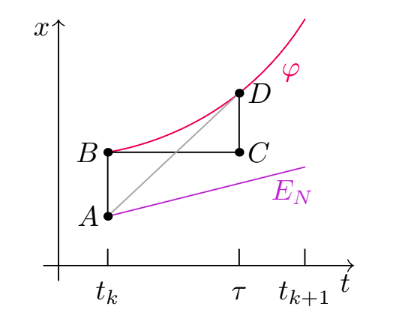
\includegraphics[scale=0.5]{Pics/Screenshot from 2021-01-14 23-23-06.png}}
\end{figure}
\begin{equation*}
    \begin{aligned}
        |(t_k, E_N(t_k)) - (\tau, \varphi(\tau))| &\le |(t_k, E_N(t_k)) - (t_k, \varphi(t_k))| + |(t_k, \varphi(t_k)) - (\tau, \varphi(t_k))| + |(\tau, \varphi(t_k)) - (\tau, \varphi(\tau))| =\\
        &= |E_N(t_k) - \varphi(t_k)| + |t_k - \tau| + |\varphi(t_k) - \varphi(\tau)|
    \end{aligned}
\end{equation*}

Каждое из трех слагаемых можно сделать меньше $\frac{\delta}{3}$ при всех достаточно больших $N$: первое слагаемое --- в силу равномерной сходимости $E_N$ к $\varphi$, второе слагаемое --- в силу того, что оно не превосходит $\frac{h}{N}$, третье слагаемое --- в силу равномерной непрерывности $\varphi$ на $[0, h]$. Отсюда следует (\ref{eulerineq}), что и завершает доказательство теоремы.
